\documentclass[a4paper]{article} % Document type

\ifx\pdfoutput\undefined
%Use old Latex if PDFLatex does not work
\usepackage[dvips]{graphicx}% To get graphics working
\DeclareGraphicsExtensions{.eps} % Encapsulated PostScript
\else
%Use PDFLatex
\usepackage[pdftex]{graphicx}% To get graphics working
\DeclareGraphicsExtensions{.pdf,.jpg,.png,.mps} % Portable Document Format, Joint Photographic Experts Group, Portable Network Graphics, MetaPost
\pdfcompresslevel=9
\fi

\usepackage[bookmarks=true,bookmarksnumbered=true,hypertexnames=true,breaklinks=true,colorlinks=true]{hyperref}
\usepackage{amsmath,amssymb}   % Contains mathematical symbols
\usepackage[ansinew]{inputenc} % Input encoding, identical to Windows 1252
\usepackage[english]{babel}    % Language
%\usepackage[round,authoryear]{natbib}  %Nice author (year) citations
%\usepackage[square,numbers]{natbib}     %Nice numbered citations
%paragraph{unsrtnat}           %Unsorted bibliography
%paragraph{plainnat}            %Sorted bibliography

\addtolength{\topmargin}{-20mm}% Removes 30mm from the top margin
\addtolength{\textheight}{10mm}% Adds it to the text height


\begin{document}               % Begins the document
	
	\title{Information Retrieval Report}
	\author{First name Last name \\ student number \\ email} 
	%\date{2010-10-10}             % If you want to set the date yourself.
	
	\maketitle                     % Generates the title
	
	
	
	
	%%%%%%%%%%%%%%%%%%%%%%%%%%%%%%%%%%%%%%%%%%%%%%%%%%%%%%%%%%%%%%%%%%%%%%%%%%%%%%%%%%%
	% Abstract of the whole project
	%%%%%%%%%%%%%%%%%%%%%%%%%%%%%%%%%%%%%%%%%%%%%%%%%%%%%%%%%%%%%%%%%%%%%%%%%%%%%%%%%%%
	
	\subsection*{Background}
	\label{background}
	
	Whole project is seperaed to four major parts:
	\begin{enumerate}
		\item Create a data base of open access full text articles responded by team Wolverine
		\item Create a complementary XML structure for metadata that contains all information in the PDF and can be show in Utopia responded by team Eagle unit
		\item Automatic creation of metadata/markup by use of natural language processing of full text articles responded by team Union
		\item Automatic creation of links from full text articles to external sources responded by team Hanky Phanky
	\end{enumerate}
	
	\clearpage
	%%%%%%%%%%%%%%%%%%%%%%%%%%%%%%%%%%%%%%%%%%%%%%%%%%%%%%%%%%%%%%%%%%%%%%%%%%%%%%%%%%%
	% Responsibility of Wolverine
	%%%%%%%%%%%%%%%%%%%%%%%%%%%%%%%%%%%%%%%%%%%%%%%%%%%%%%%%%%%%%%%%%%%%%%%%%%%%%%%%%%%
	
	\subsection*{Create a data base of open access full text article}
	\label{task1}
	
	Goal for this subsection is to build up a database which downloads articles from open access databases using web crawler or web robot. And setting up a system that can allow the users to access the data in our database. I'd like to seperate this subsection into six features, then I'll give several suggestions based on each feature. 
	
	\paragraph*{Feature 1 --Administrator}
	\label{task1:part1}
	
	In this part, the main consideration is the relationship between user and administrator. As an administrator's point, I'd like to give the best product to the consumer. On the other hand, users want to have convenient searching engine to get in touch with the knowledge. For this purpose, I'm pressure to show two suggestions for enhancing the relationship between users and producers. First, set up a popular-word-ranking system. When I search in something I don't know its name but know it in some specific area, such as stem cell in medical area. In this moment, the popular-word-ranking system will help me searching by giving me some keywords. Then, I would be easily to use this database. Of course, the popular-word-ranking system is based on users' searches and experts'suggestions to change the key words. So, the system can be trusted. 
	
	Second, build up an area in the database and let user to change the area to what they want it to be. The idea is referenced from well-known media, Wikimedia. It's so called "personalized searching". By doing this, it would help user idealize the system to what they want and suggest administrator the service which clients really want. It would lead to a win-win situation.
	
	\paragraph*{Feature 2 -- Web Crawler}
	\label{task1:feature2}
	
	The web crawler is a algorithm that has ability to quickly and accurately process and update a very large amount of data which are constantly being updated.\cite{Liu2012} It starts with a list of URLs to visit, called the seeds. As the crawler visits these URLs, it identifies all the hyperlinks in the page and adds them to the list of URLs to visit, called the crawl frontier. URLs from the frontier are recursively visited according to a set of policies. If the crawler is performing archiving of websites it copies and saves the information as it goes. The archives are usually stored in such a way they can be viewed, read and navigated as they were on the live web, but are preserved as �snapshots'.\cite{Du2013} We need to build up a web crawler to automatically visit a list of web page. Then find out which link in the page is valuable to download it into our database. 
	
	\paragraph*{Feature 3 -- User account}
	\label{task1:feature3}
	
	In this part, the main issue is how to create a user account that can connect between user and database. But the more important thing is to make sure database will not collapse by user who is not allowed to access to core part of database.
	
	To protect the database system security and privilege, this study introduces two methods for user account, principle of least privilege and role-based access control respectively. The principle of least privilege, also known as the principle of minimal privilege, means giving a user account only those those privileges which are essential to that users work \cite{PrincipleLeastPrivilege}. The role-based access control is a policy neutral access control mechanism defined around privileges and roles. It can implement discretionary access control (DAC) or mandatory access control (MAC). The role-based access control is very easy to do user assignments as the components of this policy, such as role-permissions, etc. That is why it sometimes referred to as role-based security \cite{RoleBasedAccessControl}. The information and resources would not in danger due to these two methods will filter user depend on their authority and only allow the legitimate user to access.	
	To protect the database system security and privilege, this study introduces two methods for user account, principle of least privilege and role-based access control respectively. The principle of least privilege, also known as the principle of minimal privilege, means giving a user account only those those privileges which are essential to that user`s work \cite{PrincipleLeastPrivilege}. The role-based access control is a policy neutral access control mechanism defined around privileges and roles. It can implement discretionary access control (DAC) or mandatory access control (MAC). The role-based access control is very easy to do user assignments as the components of this policy, such as role-permissions, etc. That is why it sometimes referred to as role-based security \cite{RoleBasedAccessControl}. The information and resources would not in danger due to these two methods will filter user depend on their authority and only allow the legitimate user to access.
	
	\paragraph*{Feature 4 -- User Interface}
	\label{task1:feature4}
	
	Understanding the types of visualizations people create by themselves for personal use. As part of this recent direction, we have studied a large collection of whiteboards in a research institution, where people make active use of combinations of words, diagrams and various types of visuals to help them further their thought processes. Our goal is to arrive at a better understanding of the nature of visuals that are created spontaneously during brainstorming, thinking, communicating, and general problem solving on whiteboards.\cite{Blascheck2016} We use the qualitative approaches of open coding, interviewing, and affinity diagramming to explore the use of recognizable and novel visuals, and the interplay between visualization and diagrammatic elements with words, numbers and labels. We discuss the potential implications of our findings on information visualization design. Combining the advantage of visual thinking new standard of data processing, that visual nature of computers can challenge the first generation of hackers, An icon is an image, picture, or symbol representing a concept.\cite{Szpunar2010}
	
	\paragraph*{Feature 5 -- Data Storage and Search Methods}
	\label{task1:feature5}
	
	The organization of data inside a database management system(DBMS) and retrieval methods is based on the database storage structure such as tables and indexes. 
	There are several types of database storage structure such as XML, a textual data format. 
	This advantage is self-describing and flexible in organizing data.\cite{ISI:000253400700005}Several considerations of data storage include right space allocation techniques, data compression techniques (if necessary), security and encryption and the access path to retrieve the data. 
	Therefore, DBMS software will provide some method to optimize and  minimum storage space of a database.
	
	\paragraph*{Feature 6 -- Database Management Systems}
	\label{task1:feature6}
	
	The relational database model was proposed by Edgar Codd in 1970, but because of the technological requirements it was not universal at that time. It was until 1980s that the first commercial relational database management systems began to appear. 
	A database management system (DBMS) is a computer software application that interacts with the user, other applications, and the database itself to capture and analyze data. Well-known DBMSs include MySQL, PostgreSQL, Microsoft SQL Server, Oracle, Sybase and IBM DB2. 
	Queries are the main way in which users retrieve information from a database. Most database management systems use a standard system called Structured Query Language (SQL) to query their tables. SQL is a structured form of English and resembles many programming languages, although most systems provide a graphical user-interface to generate the SQL code. And the most popular database systems since the 1980s have all supported the relational model as represented by the SQL language.\cite{Martinez-Cruz2011}	
	
	\begin{figure*}[h] % The * makes the figure span both columns, p places the figure on a float page
		\begin{center}
			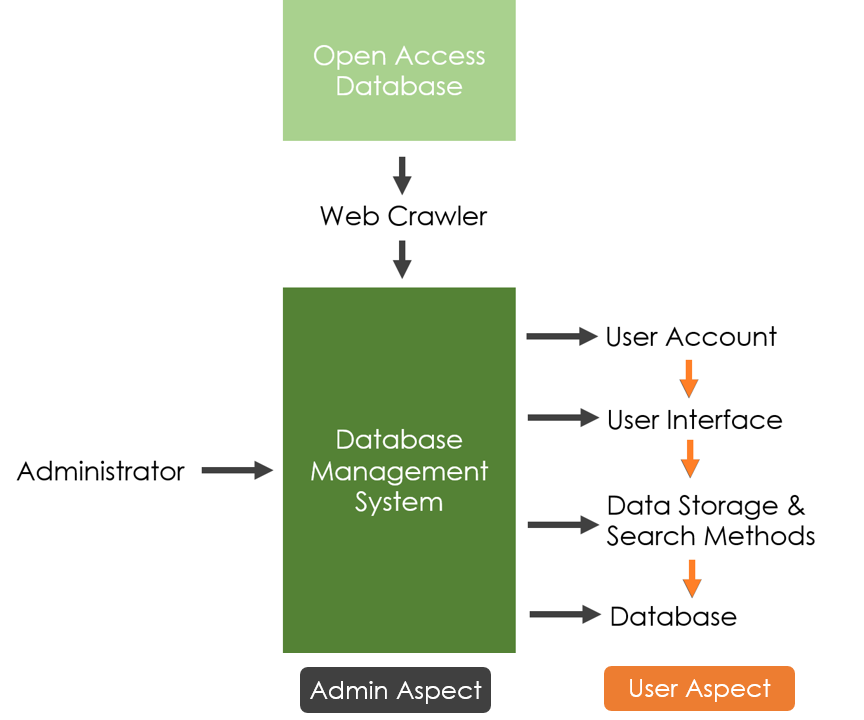
\includegraphics[scale=1.0]{WolverineChart}
		\end{center}
		\caption{Hierarchical overview}
	\end{figure*}
	\clearpage
	
	%%%%%%%%%%%%%%%%%%%%%%%%%%%%%%%%%%%%%%%%%%%%%%%%%%%%%%%%%%%%%%%%%%%%%%%%%%%%%%%%%%%
	% Responsibility of Eagle unit
	%%%%%%%%%%%%%%%%%%%%%%%%%%%%%%%%%%%%%%%%%%%%%%%%%%%%%%%%%%%%%%%%%%%%%%%%%%%%%%%%%%%
	
	\subsection*{XML metadata structure}
	\label{sec:abs}
		
	Our responsipility is to construct an XML metadata structure.	
	
	%%%%%%%%%%%%%%%%%%%%%%%%%%%%%%%%%%%%%%%%%%%%%%%%%%%%%%%%%%%%%%%%%%%%%%%%%%%%%%%%%%%
	% 1. Different standards of metadata
	%%%%%%%%%%%%%%%%%%%%%%%%%%%%%%%%%%%%%%%%%%%%%%%%%%%%%%%%%%%%%%%%%%%%%%%%%%%%%%%%%%%
	
	\paragraph*{1. Different standards of metadata}
	\label{sec:mets}
	There's many different standards existing to describe the metadata in different fields and applications. We list 5 of them and give a brief introduction to each one.
	
	\begin{enumerate}
		\item IAFA/Whois++ Templates\\
		Internet Anonymous Ftp Archive (IAFA) templates were designed to facilitate effective access to ftp (file transfer protocol) archives by means of describing the contents and services available from the archive.	
		
		\item MARC\\
		MARC was a means to allow the exchange of catalogue records between co-operating libraries, it was a format for national bibliographies to use for printed bibliographic records, and it was used by bibliographic agencies for their supply of records to libraries.
		
		\item Text Encoding Initiative (TEI)\\
		It describes the goal of the project as "to define a set of generic guidelines for the representation of textual materials in electronic form, in such a way as to enable researchers in any discipline to interchange and re-use resources, independently of software, hardware, and application area.�	
		
		\item Dublin Core\\
		The Dublin Core workshop recognised that widespread indexing and bibliographic control of Internet resources depends on the existence of a simple record to describe networked resources. The objective was to define a simple set of data elements so that authors and publishers of Internet documents could create their own metadata records in a distributed way.
		
		\item IEEE Learning Object Metadata (LOM)\\
		The LOM data schema specifies which characteristics of a learning object should be described and what vocabularies may be used for these descriptions; it also defines how this data model can be amended by additions or constraints.	
	\end{enumerate}
	
	More detailed introduction could be found in {\bf\cite{Barker:2010:metadataforlearningmaterials}} and {\bf\cite{Rachel:2009:reviewofmetadataformats}}.
	
	%%%%%%%%%%%%%%%%%%%%%%%%%%%%%%%%%%%%%%%%%%%%%%%%%%%%%%%%%%%%%%%%%%%%%%%%%%%%%%%%%%%
	% 2. Necessary elements of XML metadata
	%%%%%%%%%%%%%%%%%%%%%%%%%%%%%%%%%%%%%%%%%%%%%%%%%%%%%%%%%%%%%%%%%%%%%%%%%%%%%%%%%%%
	
	\paragraph*{2. Necessary elements of XML metadata with DTD}
	\label{sec:mets}
	{\bf\cite{Ruey-Shun:2003:DevelopinganXMLframeworkformetadatasystem}} suggest that an XML metadata discribed according the DTD include three necessary elements:
	\begin{enumerate}
		\item Structure\\
		The major execution ability of structure includes parser for well-formed XML and
		valid DTD structure, authoring tool for editing.
		
		\item Depth\\
		Basically, there are two sorts of fields: Fixed-length fields and variable fields.
		Fixed-length fields are general types and character-indication types Sub-field, whether
		fixed-length fields or variable fields, might contain both fixed-length fields and
		variable fields. According to the reason above, the process ability of the system has to
		cover the situation
		
		\item Scope\\
		The connections must involve simple object, time, space, people, and event. 
	\end{enumerate}
	%%%%%%%%%%%%%%%%%%%%%%%%%%%%%%%%%%%%%%%%%%%%%%%%%%%%%%%%%%%%%%%%%%%%%%%%%%%%%%%%%%%
	% 3. Other apllications
	%%%%%%%%%%%%%%%%%%%%%%%%%%%%%%%%%%%%%%%%%%%%%%%%%%%%%%%%%%%%%%%%%%%%%%%%%%%%%%%%%%%
	
	\paragraph*{3. Other apllications of XML metadata}
	Here's a few of useful tools and applications for XML metadata:
	\begin{enumerate}
		\item METS:\\
		METS is an XML document format intended for the encoding of complex objects within digital libraries. It provides the means to record all of the descriptive, administrative, structural and behavioral metadata needed to manage and provide access to complex digital content (McDonough2006). METS provides a method for aggregating all the metadata that can be used with a digital object. ({\bf \cite{Sharon Cheslow:2014:METSForTheCulturalHeritageCommunity}})
		
		\item PREMIS:\\
		PREservation Metadata: Implementation Strategies (PREMIS) {\bf(wiki)} is an administrative metadata schema used for the preservation of digital resources ({\bf \cite{Sharon Cheslow:2014:METSForTheCulturalHeritageCommunity}}). With the rapid changes in technology, digital objects including its metadata a bound to go obsolete at some time in the future. PREMIS was created to set standards that will ensure long term usability of digital resources. 
		
		\item MODS:\\
		Metadata Object and Description Schema (MODS) is a standard for encoding metadata of digital objects using XML. MODS among XML base metadata standards has remain the most descriptive and has high level compatibility with MARC ({\bf \cite{Rebecca Guenther:2003:NewMetadataStandardsforDigitalResources}}).
		
	\end{enumerate}
	\begin{figure*}[h] % The * makes the figure span both columns, p places the figure on a float page
		\begin{center}
			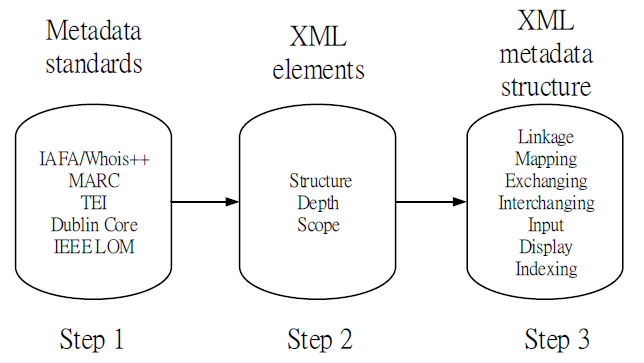
\includegraphics[scale=0.7]{EagleUnit}
		\end{center}
		\caption{Hierarchical overview}
	\end{figure*}
	\clearpage
	
	%%%%%%%%%%%%%%%%%%%%%%%%%%%%%%%%%%%%%%%%%%%%%%%%%%%%%%%%%%%%%%%%%%%%%%%%%%%%%%%%%%%
	%Automatic creation of metadata/markup by useof natural language processing of full text articles
	%%%%%%%%%%%%%%%%%%%%%%%%%%%%%%%%%%%%%%%%%%%%%%%%%%%%%%%%%%%%%%%%%%%%%%%%%%%%%%%%%%%
	
	\subsection*{overview}
	\label{task1}
	We're  producing  a  program  which  automatically  generate  metadata  such  asauthors' name,  date of publishing,  name of articles. . .   and more importantlyauto-abstract for full text articles We are interested in features for either moreconvenient use of the program or improving precise data generation There are5 related problems.
	
	
	\paragraph*{Feature 1 }
	\label{task1:feature1}
	When users search with a sentence, how do the program understand the certaininput of text?
	
	Building a natural language understanding (NLU) system.
	Use a set of possible yes-no questions that can be applied to data items, thenfollow a rule for selecting the best question at any node on the basis of trainingdata, which has a method for pruning trees to prevent over-training.
	
	\paragraph*{Feature 2 }
	\label{task1:feature2}
	
	When users search Turkey, the results could be a country or an animal.  Some-times, the results are totally unrelated.
	It's  signifcantly  crucial  for  search  engine  to  understand  what  users  want  byname  recognition  in  natural  language  processing.   Digital  libraries  and  webresources have limited metadata, augmenting them with meaningful, stable anddesired categories.  Information can enable better overviews and support userexploration
	\paragraph*{Feature 3 }
	\label{task1:feature3}
	Word sense disambiguation
	word sense disambiguation is an important step in natural language processing.This is the step where words with different meaning will be listed in different category (Abualhaija and Zimmermann, 2016). WSD has been done with threemain approaches: supervised disambiguation (Abualhaija  and  Zimmermann,2016), semi-supervised approach (Ben Aouicha et al., 2016), and more recently unsupervised approach (Yoon et al., 2006). Research for unsupervised approach has been developed quickly and application of this approach has been found in WSD for not-so-popular language such as Korean.
	
	The project team has decided to pursuit the unsupervised approach.  Implemen-tation will be made in term of symnonym grouping (Navigli, 2009) and contextclustering (Wang et al., 2009)
	
	
	\paragraph*{Feature 4 }
	\label{task1:feature4}
	The readers do not know what the connected words meaning
	Compute and Analyze in natural language processing
	I suggest we should use the Python language to complete this task.  It can easilyconpute and analyze the words in the articles.  Phthon can compute and analyzeby separating the connected words.  The readers can know what do the wordsmean when they are reading the articles .
	
	
	\paragraph*{Feature 5 }
	\label{task1:feature5}
	Natural language processing help us extract the important information from the full text article. How could we make it more efficiently and precisely?
	Query reduction to single sub-query.he performance of the machine is better in the short query rather than long query. Thus, it is an important issue to reduce the query to many sub-query. The first is extracting the single sub-query by the existing features.  Then, We combine these features to the reduction's technique. We couldn't that it is more efficient than just analyze the original query.
	\clearpage
	
	
	%%%%%%%%%%%%%%%%%%%%%%%%%%%%%%%%%%%%%%%%%%%%%%%%%%%%%%%%%%%%%%%%%%%%%%%%%%%%%%%%%%%
	% Responsibility of Hanky Phanky
	%%%%%%%%%%%%%%%%%%%%%%%%%%%%%%%%%%%%%%%%%%%%%%%%%%%%%%%%%%%%%%%%%%%%%%%%%%%%%%%%%%%
	
	\subsection*{Hanky Panky -- Background}
	\label{task1}
	
	Nowadays Internet technology push lots of information be generated. These huge among of information is impossible for human to read each of them. So lots of information retrieval technology had been developed. Text categorization systems are one of them. It is useful in a wide variety of tasks, such as routing news and e-mails. In order to identifying junk email, or handling intelligence reports. There are many techniques to approach the goal, such as support vector machines, k-nearest neighbor algorithm, and neural networks.
	
	According to \cite{Gabrilovich:2007:HEH:1314498.1314573}, one of the early method is bag of words (BOW). The features commonly used are the individual words appearing in the training documents, and the order of the words is ignored. The value of a feature for a particular document is usually its occurrence frequency. Although this representation scheme is easy and efficiency,  there are still some disadvantage. One of them is treating each document as a bag of the words, and is therefore known as the bag of words (BOW) approach (Salton and McGill, 1983).
	
	To improve the accuracy, there have been a number of methods to add outside knowledge to effect machine learning techniques. Transfer learning approaches (Bennett et al., 2003; Do and Ng, 2005; Sutton and McCallum, 1998; Raina et al., 2006) employ information from some related learning tasks. Pseudo-relevance feedback (Ruthven and Lalmas, 2003) use information of several top-ranked documents. Semi-supervised methods (Goldberg and Zhu, 2006; Ando and Zhang, 2005a,b; Blei et al., 2003; Nigam et al., 2000; Joachims, 1999b) help to infer information from unlabeled data, because is more available than labeled data. \cite{Gabrilovich:2007:HEH:1314498.1314573} introduce a method for enhancing machine learning algorithms with a large volume of extracted knowledge, mainly by existing induction techniques while enriching the language of representation, namely, exploring new feature spaces. In \cite{ISI:000295620300006} resent a classification of all conflation processes of geospatial databases from heterogeneous sources.
	\clearpage
	
	%%%%%%%%%%%%%%%%%%%%%%%%%%%%%%%%%%%%%%%%%%%%%%%%%%%%%%%%%%%%%%%%%%%%%%%%%%%%%%%%%%%
	% The bibliography
	%%%%%%%%%%%%%%%%%%%%%%%%%%%%%%%%%%%%%%%%%%%%%%%%%%%%%%%%%%%%%%%%%%%%%%%%%%%%%%%%%%%
	
	%% I would strongly recommend you to use Mendeley desktop or a similar reference manager 
	%% that can generate a bibtex file so that you don't need to insert references manually. 
	%% It will save you a lot of time. Bests, Prof. Nordling
	
	\bibliographystyle{plain}
	\bibliography{library}
	
	%%%%%%%%%%%%%%%%%%%%%%%%%%%%%%%%%%%%%%%%%%%%%%%%%%%%%%%%%%%%%%%%%%%%%%%%%%%%%%%%%%%
	% Place your figures and tables at the end of the document starting on a new page
	%%%%%%%%%%%%%%%%%%%%%%%%%%%%%%%%%%%%%%%%%%%%%%%%%%%%%%%%%%%%%%%%%%%%%%%%%%%%%%%%%%%
	\clearpage % Ends the current page and causes all figures and tables to be printed
	
\end{document}      % End of the document
